% Options for packages loaded elsewhere
\PassOptionsToPackage{unicode}{hyperref}
\PassOptionsToPackage{hyphens}{url}
\PassOptionsToPackage{dvipsnames,svgnames,x11names}{xcolor}
%
\documentclass[
]{article}

\usepackage{amsmath,amssymb}
\usepackage{iftex}
\ifPDFTeX
  \usepackage[T1]{fontenc}
  \usepackage[utf8]{inputenc}
  \usepackage{textcomp} % provide euro and other symbols
\else % if luatex or xetex
  \usepackage{unicode-math}
  \defaultfontfeatures{Scale=MatchLowercase}
  \defaultfontfeatures[\rmfamily]{Ligatures=TeX,Scale=1}
\fi
\usepackage{lmodern}
\ifPDFTeX\else  
    % xetex/luatex font selection
\fi
% Use upquote if available, for straight quotes in verbatim environments
\IfFileExists{upquote.sty}{\usepackage{upquote}}{}
\IfFileExists{microtype.sty}{% use microtype if available
  \usepackage[]{microtype}
  \UseMicrotypeSet[protrusion]{basicmath} % disable protrusion for tt fonts
}{}
\makeatletter
\@ifundefined{KOMAClassName}{% if non-KOMA class
  \IfFileExists{parskip.sty}{%
    \usepackage{parskip}
  }{% else
    \setlength{\parindent}{0pt}
    \setlength{\parskip}{6pt plus 2pt minus 1pt}}
}{% if KOMA class
  \KOMAoptions{parskip=half}}
\makeatother
\usepackage{xcolor}
\setlength{\emergencystretch}{3em} % prevent overfull lines
\setcounter{secnumdepth}{-\maxdimen} % remove section numbering
% Make \paragraph and \subparagraph free-standing
\makeatletter
\ifx\paragraph\undefined\else
  \let\oldparagraph\paragraph
  \renewcommand{\paragraph}{
    \@ifstar
      \xxxParagraphStar
      \xxxParagraphNoStar
  }
  \newcommand{\xxxParagraphStar}[1]{\oldparagraph*{#1}\mbox{}}
  \newcommand{\xxxParagraphNoStar}[1]{\oldparagraph{#1}\mbox{}}
\fi
\ifx\subparagraph\undefined\else
  \let\oldsubparagraph\subparagraph
  \renewcommand{\subparagraph}{
    \@ifstar
      \xxxSubParagraphStar
      \xxxSubParagraphNoStar
  }
  \newcommand{\xxxSubParagraphStar}[1]{\oldsubparagraph*{#1}\mbox{}}
  \newcommand{\xxxSubParagraphNoStar}[1]{\oldsubparagraph{#1}\mbox{}}
\fi
\makeatother
\usepackage{color}
\usepackage{fancyvrb}
\newcommand{\VerbBar}{|}
\newcommand{\VERB}{\Verb[commandchars=\\\{\}]}
\DefineVerbatimEnvironment{Highlighting}{Verbatim}{commandchars=\\\{\}}
% Add ',fontsize=\small' for more characters per line
\usepackage{framed}
\definecolor{shadecolor}{RGB}{241,243,245}
\newenvironment{Shaded}{\begin{snugshade}}{\end{snugshade}}
\newcommand{\AlertTok}[1]{\textcolor[rgb]{0.68,0.00,0.00}{#1}}
\newcommand{\AnnotationTok}[1]{\textcolor[rgb]{0.37,0.37,0.37}{#1}}
\newcommand{\AttributeTok}[1]{\textcolor[rgb]{0.40,0.45,0.13}{#1}}
\newcommand{\BaseNTok}[1]{\textcolor[rgb]{0.68,0.00,0.00}{#1}}
\newcommand{\BuiltInTok}[1]{\textcolor[rgb]{0.00,0.23,0.31}{#1}}
\newcommand{\CharTok}[1]{\textcolor[rgb]{0.13,0.47,0.30}{#1}}
\newcommand{\CommentTok}[1]{\textcolor[rgb]{0.37,0.37,0.37}{#1}}
\newcommand{\CommentVarTok}[1]{\textcolor[rgb]{0.37,0.37,0.37}{\textit{#1}}}
\newcommand{\ConstantTok}[1]{\textcolor[rgb]{0.56,0.35,0.01}{#1}}
\newcommand{\ControlFlowTok}[1]{\textcolor[rgb]{0.00,0.23,0.31}{\textbf{#1}}}
\newcommand{\DataTypeTok}[1]{\textcolor[rgb]{0.68,0.00,0.00}{#1}}
\newcommand{\DecValTok}[1]{\textcolor[rgb]{0.68,0.00,0.00}{#1}}
\newcommand{\DocumentationTok}[1]{\textcolor[rgb]{0.37,0.37,0.37}{\textit{#1}}}
\newcommand{\ErrorTok}[1]{\textcolor[rgb]{0.68,0.00,0.00}{#1}}
\newcommand{\ExtensionTok}[1]{\textcolor[rgb]{0.00,0.23,0.31}{#1}}
\newcommand{\FloatTok}[1]{\textcolor[rgb]{0.68,0.00,0.00}{#1}}
\newcommand{\FunctionTok}[1]{\textcolor[rgb]{0.28,0.35,0.67}{#1}}
\newcommand{\ImportTok}[1]{\textcolor[rgb]{0.00,0.46,0.62}{#1}}
\newcommand{\InformationTok}[1]{\textcolor[rgb]{0.37,0.37,0.37}{#1}}
\newcommand{\KeywordTok}[1]{\textcolor[rgb]{0.00,0.23,0.31}{\textbf{#1}}}
\newcommand{\NormalTok}[1]{\textcolor[rgb]{0.00,0.23,0.31}{#1}}
\newcommand{\OperatorTok}[1]{\textcolor[rgb]{0.37,0.37,0.37}{#1}}
\newcommand{\OtherTok}[1]{\textcolor[rgb]{0.00,0.23,0.31}{#1}}
\newcommand{\PreprocessorTok}[1]{\textcolor[rgb]{0.68,0.00,0.00}{#1}}
\newcommand{\RegionMarkerTok}[1]{\textcolor[rgb]{0.00,0.23,0.31}{#1}}
\newcommand{\SpecialCharTok}[1]{\textcolor[rgb]{0.37,0.37,0.37}{#1}}
\newcommand{\SpecialStringTok}[1]{\textcolor[rgb]{0.13,0.47,0.30}{#1}}
\newcommand{\StringTok}[1]{\textcolor[rgb]{0.13,0.47,0.30}{#1}}
\newcommand{\VariableTok}[1]{\textcolor[rgb]{0.07,0.07,0.07}{#1}}
\newcommand{\VerbatimStringTok}[1]{\textcolor[rgb]{0.13,0.47,0.30}{#1}}
\newcommand{\WarningTok}[1]{\textcolor[rgb]{0.37,0.37,0.37}{\textit{#1}}}

\providecommand{\tightlist}{%
  \setlength{\itemsep}{0pt}\setlength{\parskip}{0pt}}\usepackage{longtable,booktabs,array}
\usepackage{calc} % for calculating minipage widths
% Correct order of tables after \paragraph or \subparagraph
\usepackage{etoolbox}
\makeatletter
\patchcmd\longtable{\par}{\if@noskipsec\mbox{}\fi\par}{}{}
\makeatother
% Allow footnotes in longtable head/foot
\IfFileExists{footnotehyper.sty}{\usepackage{footnotehyper}}{\usepackage{footnote}}
\makesavenoteenv{longtable}
\usepackage{graphicx}
\makeatletter
\def\maxwidth{\ifdim\Gin@nat@width>\linewidth\linewidth\else\Gin@nat@width\fi}
\def\maxheight{\ifdim\Gin@nat@height>\textheight\textheight\else\Gin@nat@height\fi}
\makeatother
% Scale images if necessary, so that they will not overflow the page
% margins by default, and it is still possible to overwrite the defaults
% using explicit options in \includegraphics[width, height, ...]{}
\setkeys{Gin}{width=\maxwidth,height=\maxheight,keepaspectratio}
% Set default figure placement to htbp
\makeatletter
\def\fps@figure{htbp}
\makeatother

\makeatletter
\@ifpackageloaded{caption}{}{\usepackage{caption}}
\AtBeginDocument{%
\ifdefined\contentsname
  \renewcommand*\contentsname{Table of contents}
\else
  \newcommand\contentsname{Table of contents}
\fi
\ifdefined\listfigurename
  \renewcommand*\listfigurename{List of Figures}
\else
  \newcommand\listfigurename{List of Figures}
\fi
\ifdefined\listtablename
  \renewcommand*\listtablename{List of Tables}
\else
  \newcommand\listtablename{List of Tables}
\fi
\ifdefined\figurename
  \renewcommand*\figurename{Figure}
\else
  \newcommand\figurename{Figure}
\fi
\ifdefined\tablename
  \renewcommand*\tablename{Table}
\else
  \newcommand\tablename{Table}
\fi
}
\@ifpackageloaded{float}{}{\usepackage{float}}
\floatstyle{ruled}
\@ifundefined{c@chapter}{\newfloat{codelisting}{h}{lop}}{\newfloat{codelisting}{h}{lop}[chapter]}
\floatname{codelisting}{Listing}
\newcommand*\listoflistings{\listof{codelisting}{List of Listings}}
\makeatother
\makeatletter
\makeatother
\makeatletter
\@ifpackageloaded{caption}{}{\usepackage{caption}}
\@ifpackageloaded{subcaption}{}{\usepackage{subcaption}}
\makeatother

\usepackage{hyphenat}
\usepackage{ifthen}
\usepackage{calc}
\usepackage{calculator}



\usepackage{graphicx}
\usepackage{geometry}
\usepackage{afterpage}
\usepackage{tikz}
\usetikzlibrary{calc}
\usetikzlibrary{fadings}
\usepackage[pagecolor=none]{pagecolor}


% Set the titlepage font families







% Set the coverpage font families


\ifLuaTeX
  \usepackage{selnolig}  % disable illegal ligatures
\fi
\usepackage{bookmark}

\IfFileExists{xurl.sty}{\usepackage{xurl}}{} % add URL line breaks if available
\urlstyle{same} % disable monospaced font for URLs
\hypersetup{
  colorlinks=true,
  linkcolor={blue},
  filecolor={Maroon},
  citecolor={Blue},
  urlcolor={Blue},
  pdfcreator={LaTeX via pandoc}}


\author{}
\date{}

\begin{document}
%%%%% begin titlepage extension code


\begin{titlepage}

%%% TITLE PAGE START

% Set up alignment commands
%Page
\newcommand{\titlepagepagealign}{
\ifthenelse{\equal{left}{right}}{\raggedleft}{}
\ifthenelse{\equal{left}{center}}{\centering}{}
\ifthenelse{\equal{left}{left}}{\raggedright}{}
}


\newcommand{\titleandsubtitle}{
% Title and subtitle
}
\newcommand{\titlepagetitleblock}{
\titleandsubtitle
}

\newcommand{\authorstyle}[1]{{#1}}

\newcommand{\affiliationstyle}[1]{{#1}}

\newcommand{\titlepageauthorblock}{
{\authorstyle{}}}

\newcommand{\titlepageaffiliationblock}{
\hangindent=1em
\hangafter=1
{\affiliationstyle{


\vspace{1\baselineskip} 
}}
}
\newcommand{\headerstyled}{%
{}
}
\newcommand{\footerstyled}{%
{}
}
\newcommand{\datestyled}{%
{}
}


\newcommand{\titlepageheaderblock}{\headerstyled}

\newcommand{\titlepagefooterblock}{
\footerstyled
}

\newcommand{\titlepagedateblock}{
\datestyled
}

%set up blocks so user can specify order
\newcommand{\titleblock}{}

\newcommand{\authorblock}{}

\newcommand{\affiliationblock}{}

\newcommand{\logoblock}{}

\newcommand{\footerblock}{}

\newcommand{\dateblock}{}

\newcommand{\headerblock}{}

\thispagestyle{empty} % no page numbers on titlepages


\newlength{\minipagewidth}
\setlength{\minipagewidth}{\textwidth}
\raggedright % single minipage
% [position of box][box height][inner position]{width}
% [s] means stretch out vertically; assuming there is a vfill
\begin{minipage}[b][\textheight][s]{\minipagewidth}
\titlepagepagealign
\headerblock

\titleblock

\authorblock

\affiliationblock

\vfill

\logoblock

\footerblock
\par

\end{minipage}\ifthenelse{\equal{}{right} \OR \equal{}{leftright} }{
\hspace{\B}
\vrulecode}{}
\clearpage
%%% TITLE PAGE END
\end{titlepage}
\setcounter{page}{1}

%%%%% end titlepage extension code


\section{Data compilation for all fleets in the operating
model}\label{data-compilation-for-all-fleets-in-the-operating-model}

In this last step we will compile all of the output data files from the
different data sources (NMFS commercial trip tickets, NMFS recreational
statistics, Sea Around Us) and check the files for accuracy.

\subsection{Data upload}\label{data-upload}

First we access all of the final data files from the previous steps.

\begin{Shaded}
\begin{Highlighting}[]
\CommentTok{\# clear workspace}
\FunctionTok{rm}\NormalTok{(}\AttributeTok{list =} \FunctionTok{ls}\NormalTok{())}

\CommentTok{\# view data files in directory}
\FunctionTok{dir}\NormalTok{(}\StringTok{"data/FINAL\_files/"}\NormalTok{)}
\end{Highlighting}
\end{Shaded}

\begin{verbatim}
[1] "CAR_rep_unrep_TomFormat.csv" "commercial_TomFormat.csv"   
[3] "Intl_highseas_TomFormat.csv" "NED_Intl_TomFormat.csv"     
[5] "rec_catch_TomFormat.csv"    
\end{verbatim}

\begin{Shaded}
\begin{Highlighting}[]
\NormalTok{intc }\OtherTok{\textless{}{-}} \FunctionTok{read.csv}\NormalTok{(}\StringTok{"data/FINAL\_files/CAR\_rep\_unrep\_TomFormat.csv"}\NormalTok{)}
\NormalTok{inth }\OtherTok{\textless{}{-}} \FunctionTok{read.csv}\NormalTok{(}\StringTok{"data/FINAL\_files/Intl\_highseas\_TomFormat.csv"}\NormalTok{)}
\NormalTok{intn }\OtherTok{\textless{}{-}} \FunctionTok{read.csv}\NormalTok{(}\StringTok{"data/FINAL\_files/NED\_Intl\_TomFormat.csv"}\NormalTok{)}
\NormalTok{com }\OtherTok{\textless{}{-}} \FunctionTok{read.csv}\NormalTok{(}\StringTok{"data/FINAL\_files/commercial\_TomFormat.csv"}\NormalTok{)}
\NormalTok{rec }\OtherTok{\textless{}{-}} \FunctionTok{read.csv}\NormalTok{(}\StringTok{"data/FINAL\_files/rec\_catch\_TomFormat.csv"}\NormalTok{)}

\CommentTok{\#head(intc)}
\CommentTok{\#head(inth)}
\CommentTok{\#head(intn)}
\CommentTok{\#head(com)}
\CommentTok{\#head(rec)}

\NormalTok{d }\OtherTok{\textless{}{-}} \FunctionTok{rbind}\NormalTok{(intc, inth, intn, com, rec)}

\CommentTok{\# check for zeros and NAs}
\CommentTok{\#hist(d$Catch\_lbs)}
\FunctionTok{table}\NormalTok{(d}\SpecialCharTok{$}\NormalTok{Catch\_lbs }\SpecialCharTok{==} \DecValTok{0}\NormalTok{)}
\end{Highlighting}
\end{Shaded}

\begin{verbatim}

FALSE  TRUE 
 2078   710 
\end{verbatim}

\begin{Shaded}
\begin{Highlighting}[]
\FunctionTok{table}\NormalTok{(}\FunctionTok{is.na}\NormalTok{(d}\SpecialCharTok{$}\NormalTok{Catch\_lbs))}
\end{Highlighting}
\end{Shaded}

\begin{verbatim}

FALSE 
 2788 
\end{verbatim}

\begin{Shaded}
\begin{Highlighting}[]
\FunctionTok{apply}\NormalTok{(d, }\DecValTok{2}\NormalTok{, }\ControlFlowTok{function}\NormalTok{ (x) }\FunctionTok{table}\NormalTok{(}\FunctionTok{is.na}\NormalTok{(x)))}
\end{Highlighting}
\end{Shaded}

\begin{verbatim}
     Year   Quarter     Fleet      Area Catch_lbs 
     2788      2788      2788      2788      2788 
\end{verbatim}

\begin{Shaded}
\begin{Highlighting}[]
\CommentTok{\# resort levels geographically}
\NormalTok{d}\SpecialCharTok{$}\NormalTok{Area }\OtherTok{\textless{}{-}} \FunctionTok{factor}\NormalTok{(d}\SpecialCharTok{$}\NormalTok{Area, }\AttributeTok{levels =} \FunctionTok{c}\NormalTok{(}\StringTok{"NCA"}\NormalTok{, }\StringTok{"CAR"}\NormalTok{, }\StringTok{"FLK"}\NormalTok{, }\StringTok{"NCFL"}\NormalTok{, }\StringTok{"NNC"}\NormalTok{, }\StringTok{"VBM"}\NormalTok{, }\StringTok{"NED"}\NormalTok{))}
\NormalTok{d}\SpecialCharTok{$}\NormalTok{Fleet }\OtherTok{\textless{}{-}} \FunctionTok{factor}\NormalTok{(d}\SpecialCharTok{$}\NormalTok{Fleet, }\AttributeTok{levels =} \FunctionTok{c}\NormalTok{(}\StringTok{"Rec"}\NormalTok{, }\StringTok{"Hire"}\NormalTok{, }\StringTok{"UScom"}\NormalTok{, }\StringTok{"Intl"}\NormalTok{, }\StringTok{"UnRep"}\NormalTok{))}
\end{Highlighting}
\end{Shaded}

\subsection{Visualizing the final data
set}\label{visualizing-the-final-data-set}

We plot the final data set in a number of different ways to detect any
errors that may have occurred during processing.

\begin{Shaded}
\begin{Highlighting}[]
\CommentTok{\# plot the total catches by each factor}
\FunctionTok{par}\NormalTok{(}\AttributeTok{mfrow =} \FunctionTok{c}\NormalTok{(}\DecValTok{2}\NormalTok{, }\DecValTok{2}\NormalTok{), }\AttributeTok{mex =} \FloatTok{0.7}\NormalTok{)}
\FunctionTok{barplot}\NormalTok{(}\FunctionTok{tapply}\NormalTok{(d}\SpecialCharTok{$}\NormalTok{Catch\_lbs, d}\SpecialCharTok{$}\NormalTok{Year, sum, }\AttributeTok{na.rm =}\NormalTok{ T)}\SpecialCharTok{/}\DecValTok{10}\SpecialCharTok{\^{}}\DecValTok{6}\NormalTok{, }\AttributeTok{las =} \DecValTok{2}\NormalTok{,}
        \AttributeTok{main =} \StringTok{"Total catch by year"}\NormalTok{, }\AttributeTok{ylab =} \StringTok{"total catch (millions of pounds)"}\NormalTok{)}
\FunctionTok{barplot}\NormalTok{(}\FunctionTok{tapply}\NormalTok{(d}\SpecialCharTok{$}\NormalTok{Catch\_lbs, d}\SpecialCharTok{$}\NormalTok{Quarter, sum, }\AttributeTok{na.rm =}\NormalTok{ T)}\SpecialCharTok{/}\DecValTok{10}\SpecialCharTok{\^{}}\DecValTok{6}\NormalTok{, }
        \AttributeTok{ylab =} \StringTok{"total catch (millions of pounds)"}\NormalTok{, }\AttributeTok{main =} \StringTok{"Total catch by quarter"}\NormalTok{)}
\FunctionTok{barplot}\NormalTok{(}\FunctionTok{tapply}\NormalTok{(d}\SpecialCharTok{$}\NormalTok{Catch\_lbs, d}\SpecialCharTok{$}\NormalTok{Fleet, sum, }\AttributeTok{na.rm =}\NormalTok{ T)}\SpecialCharTok{/}\DecValTok{10}\SpecialCharTok{\^{}}\DecValTok{6}\NormalTok{, }
        \AttributeTok{main =} \StringTok{"Total catch by fleet"}\NormalTok{, }\AttributeTok{ylab =} \StringTok{"total catch (millions of pounds)"}\NormalTok{)}
\FunctionTok{barplot}\NormalTok{(}\FunctionTok{tapply}\NormalTok{(d}\SpecialCharTok{$}\NormalTok{Catch\_lbs, d}\SpecialCharTok{$}\NormalTok{Area, sum, }\AttributeTok{na.rm =}\NormalTok{ T)}\SpecialCharTok{/}\DecValTok{10}\SpecialCharTok{\^{}}\DecValTok{6}\NormalTok{, }
        \AttributeTok{main =} \StringTok{"Total catch by area"}\NormalTok{, }\AttributeTok{ylab =} \StringTok{"total catch (millions of pounds)"}\NormalTok{)}
\end{Highlighting}
\end{Shaded}

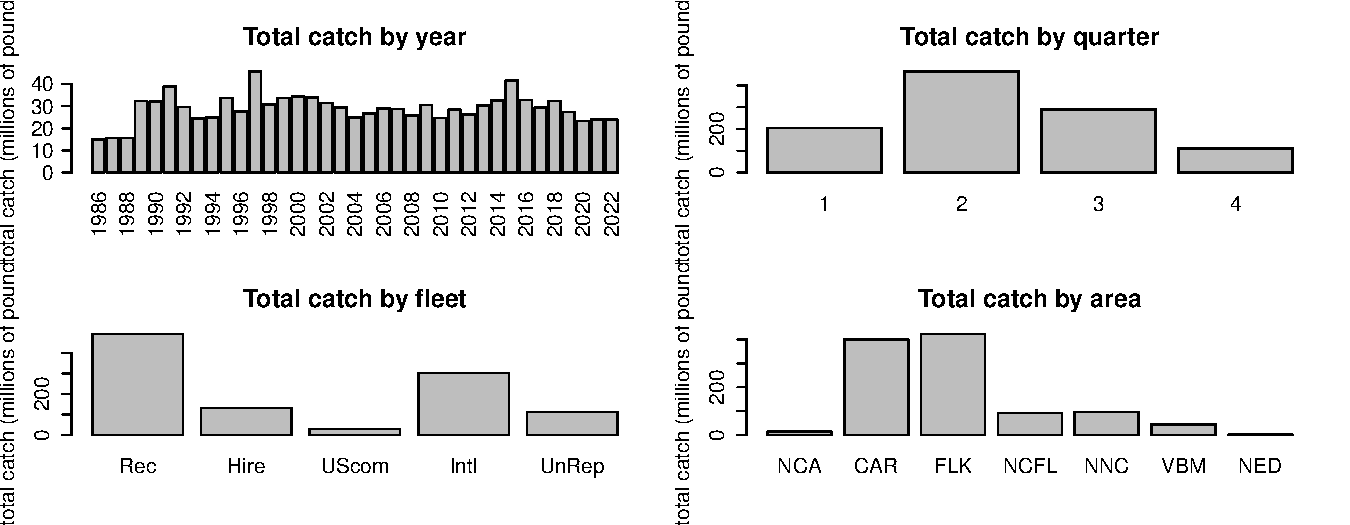
\includegraphics{compile_all_data_files/figure-pdf/unnamed-chunk-2-1.pdf}

The total catch in the regions analyzed is highly variable but
relatively stable over time with a slight decrease in recent years. Most
of the catch is caught in quarter 2 (March - May). The largest sector is
the U.S. private recreational sector, followed by international fleets
(all types), the for-hire fleet and then the U.S. commercial fleet. Most
of the fishing activity takes place in the Florida Keys and the Greater
Caribbean, with other regions contributing much less.

\begin{Shaded}
\begin{Highlighting}[]
\FunctionTok{par}\NormalTok{(}\AttributeTok{mfrow =} \FunctionTok{c}\NormalTok{(}\DecValTok{1}\NormalTok{, }\DecValTok{1}\NormalTok{))}
\NormalTok{tab }\OtherTok{\textless{}{-}} \FunctionTok{tapply}\NormalTok{(d}\SpecialCharTok{$}\NormalTok{Catch\_lbs, }\FunctionTok{list}\NormalTok{(d}\SpecialCharTok{$}\NormalTok{Fleet, d}\SpecialCharTok{$}\NormalTok{Area), sum, }\AttributeTok{na.rm =}\NormalTok{ T)}\SpecialCharTok{/}\DecValTok{10}\SpecialCharTok{\^{}}\DecValTok{6}
\FunctionTok{barplot}\NormalTok{(tab, }\AttributeTok{beside =}\NormalTok{ T, }\AttributeTok{col =} \DecValTok{2}\SpecialCharTok{:}\DecValTok{6}\NormalTok{, }\AttributeTok{legend =} \FunctionTok{rownames}\NormalTok{(tab),}
        \AttributeTok{main =} \StringTok{"Total dolphin catch by area and fleet"}\NormalTok{, }
        \AttributeTok{ylab =} \StringTok{"total catch (millions of pounds)"}\NormalTok{)}
\end{Highlighting}
\end{Shaded}

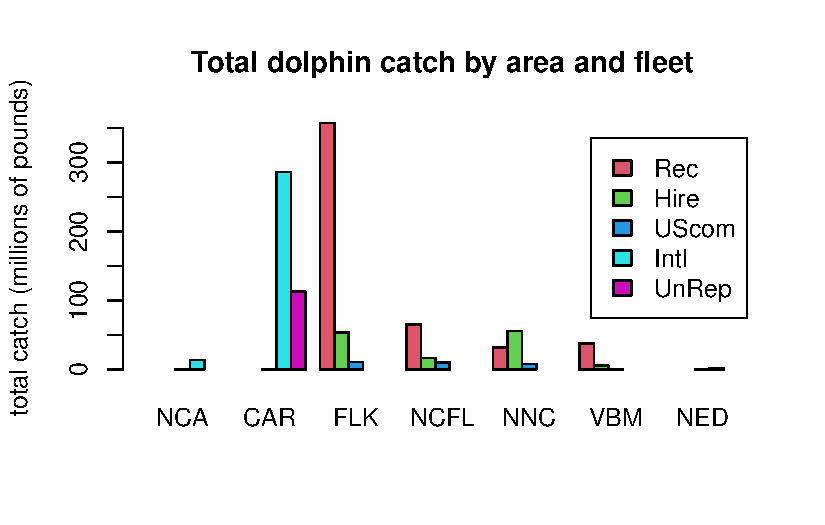
\includegraphics{compile_all_data_files/figure-pdf/unnamed-chunk-3-1.pdf}

As expected, U.S. recreational fishing (private and for-hire) only takes
place in the four U.S. EEZ regions (FLK, NCFL, NNC and VBM). The U.S.
commercial fishery operates largely in those four U.S. EEZ regions, with
small amounts of catch in the high seas of NCA, CAR and NED regions.
International catches occur largely in the Caribbean, with lesser
amounts in the NCA and NED high seas regions.

\begin{Shaded}
\begin{Highlighting}[]
\NormalTok{tab }\OtherTok{\textless{}{-}} \FunctionTok{tapply}\NormalTok{(d}\SpecialCharTok{$}\NormalTok{Catch\_lbs, }\FunctionTok{list}\NormalTok{(d}\SpecialCharTok{$}\NormalTok{Quarter, d}\SpecialCharTok{$}\NormalTok{Area), sum, }\AttributeTok{na.rm =}\NormalTok{ T)}\SpecialCharTok{/}\DecValTok{10}\SpecialCharTok{\^{}}\DecValTok{6}
\NormalTok{tabp }\OtherTok{\textless{}{-}} \FunctionTok{apply}\NormalTok{(tab, }\DecValTok{2}\NormalTok{, }\ControlFlowTok{function}\NormalTok{(x) x }\SpecialCharTok{/} \FunctionTok{sum}\NormalTok{(x, }\AttributeTok{na.rm =}\NormalTok{ T))}

\FunctionTok{barplot}\NormalTok{(tabp, }\AttributeTok{beside =}\NormalTok{ T, }\AttributeTok{col =} \FunctionTok{rainbow}\NormalTok{(}\DecValTok{4}\NormalTok{), }
        \AttributeTok{legend =} \FunctionTok{c}\NormalTok{(}\StringTok{"winter (DJF)"}\NormalTok{, }\StringTok{"spring (MAM)"}\NormalTok{, }\StringTok{"summer (JJA)"}\NormalTok{, }\StringTok{"fall (SON)"}\NormalTok{), }
        \AttributeTok{args.legend =} \FunctionTok{list}\NormalTok{(}\AttributeTok{x =} \DecValTok{15}\NormalTok{, }\AttributeTok{y =} \FloatTok{0.7}\NormalTok{, }\AttributeTok{bty =} \StringTok{"n"}\NormalTok{), }
        \AttributeTok{main =} \StringTok{"Total dolphin catch by area and season"}\NormalTok{, }
        \AttributeTok{ylab =} \StringTok{"proportion of catch)"}\NormalTok{)}
\end{Highlighting}
\end{Shaded}

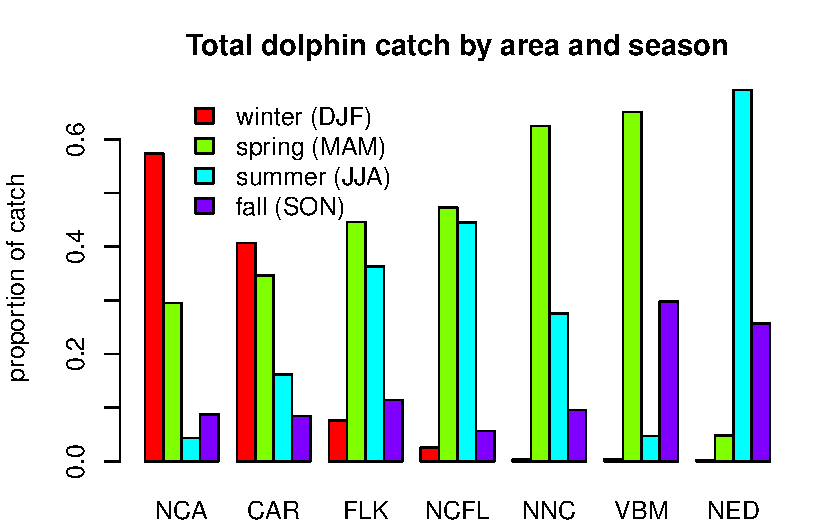
\includegraphics{compile_all_data_files/figure-pdf/unnamed-chunk-4-1.pdf}

This plot shows the seasonal movements of dolphin across the different
regions, as expressed through the proportion of catch that occurs in
each quarter within each area. In the NCA and CAR regions, most of the
catch occurs in winter, whereas in the U.S. South Atlantic regions, most
of the catch occurs in spring and summer. In the U.S. Mid-Atlantic the
catch also occurs largely in spring, and also fall. In the NED region
most of the catch occurs in summer.

\begin{Shaded}
\begin{Highlighting}[]
\NormalTok{tab }\OtherTok{\textless{}{-}} \FunctionTok{tapply}\NormalTok{(d}\SpecialCharTok{$}\NormalTok{Catch\_lbs, }\FunctionTok{list}\NormalTok{(d}\SpecialCharTok{$}\NormalTok{Year, d}\SpecialCharTok{$}\NormalTok{Fleet), sum, }\AttributeTok{na.rm =}\NormalTok{ T)}\SpecialCharTok{/}\DecValTok{10}\SpecialCharTok{\^{}}\DecValTok{6}

\FunctionTok{matplot}\NormalTok{(}\FunctionTok{rownames}\NormalTok{(tab), tab, }
        \AttributeTok{col =} \FunctionTok{c}\NormalTok{(}\StringTok{"navy"}\NormalTok{, }\StringTok{"blue"}\NormalTok{, }\StringTok{"darkturquoise"}\NormalTok{, }\StringTok{"red"}\NormalTok{, }\StringTok{"pink"}\NormalTok{), }
        \AttributeTok{type =} \StringTok{"l"}\NormalTok{, }\AttributeTok{lwd =} \DecValTok{2}\NormalTok{, }\AttributeTok{lty =} \FunctionTok{c}\NormalTok{(}\FunctionTok{rep}\NormalTok{(}\DecValTok{1}\NormalTok{, }\DecValTok{3}\NormalTok{), }\DecValTok{2}\NormalTok{, }\DecValTok{2}\NormalTok{), }
        \AttributeTok{main =} \StringTok{"Total annual dolphin catch by fleet"}\NormalTok{, }\AttributeTok{xlab =} \StringTok{""}\NormalTok{,}
        \AttributeTok{ylab =} \StringTok{"total catch (millions of pounds)"}\NormalTok{)}
\FunctionTok{legend}\NormalTok{(}\StringTok{"top"}\NormalTok{, }\AttributeTok{lwd =} \DecValTok{2}\NormalTok{, }\AttributeTok{lty =} \FunctionTok{c}\NormalTok{(}\FunctionTok{rep}\NormalTok{(}\DecValTok{1}\NormalTok{, }\DecValTok{3}\NormalTok{), }\DecValTok{2}\NormalTok{, }\DecValTok{2}\NormalTok{), }\AttributeTok{bty =} \StringTok{"n"}\NormalTok{, }
       \FunctionTok{c}\NormalTok{(}\StringTok{"U.S. private rec"}\NormalTok{, }\StringTok{"U.S. for{-}hire"}\NormalTok{, }\StringTok{"U.S. commercial"}\NormalTok{, }
         \StringTok{"International"}\NormalTok{, }\StringTok{"Unreported"}\NormalTok{),}
       \AttributeTok{col =} \FunctionTok{c}\NormalTok{(}\StringTok{"navy"}\NormalTok{, }\StringTok{"blue"}\NormalTok{, }\StringTok{"darkturquoise"}\NormalTok{, }\StringTok{"red"}\NormalTok{, }\StringTok{"pink"}\NormalTok{))}
\end{Highlighting}
\end{Shaded}

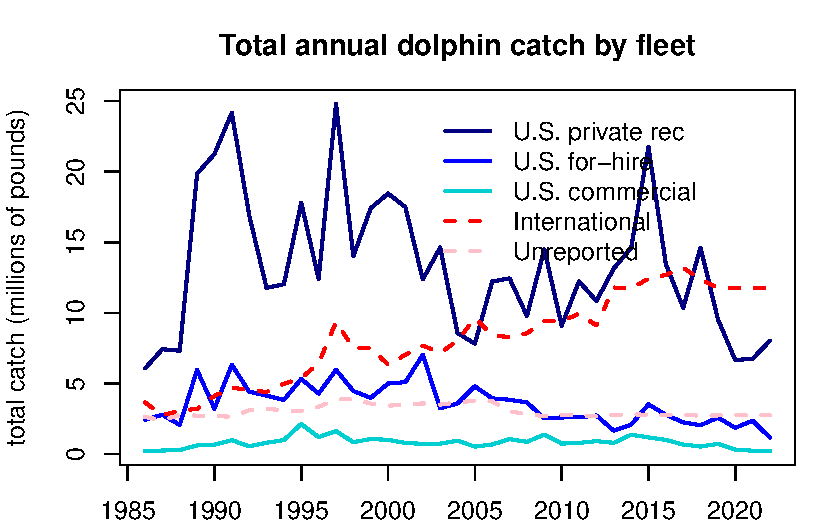
\includegraphics{compile_all_data_files/figure-pdf/unnamed-chunk-5-1.pdf}

This plot shows the time series of total annual dolphin catches by
fleet. We can compare these figures with the plots from the previous
chapters to ensure the data were processed correctly. The magnitude and
variability of the landings match the expectations.

\subsection{Distribute the high seas landings across quarters of the
year}\label{distribute-the-high-seas-landings-across-quarters-of-the-year}

The international landings are only reported as annual catches and do
not have any month or season associated with them. However, the MSE
operating model requires seasonal catches. The majority of the
international landings are caught by longline, so we will assume that
the fleet distribution of the U.S. pelagic longline is representative of
the seasonality of the international high seas fleets. Now we parse the
annual catches according to the seasonality of the U.S. fleet.

At the time of analysis, the SAU database only contained catches to
2019, so we interpolated the 2019 values to cover years 2020 - 2022.

Finally, we format the data in the format for input into the operating
model.

\begin{Shaded}
\begin{Highlighting}[]
\FunctionTok{write.csv}\NormalTok{(d, }\AttributeTok{file =} \StringTok{"data/FINAL\_files/complete\_catch\_dataset\_09052025.csv"}\NormalTok{, }\AttributeTok{row.names =} \ConstantTok{FALSE}\NormalTok{)}
\end{Highlighting}
\end{Shaded}





\end{document}
